%
\documentclass[usenames,dvipsnames]{beamer}

\usepackage{graphicx}
\usepackage{tikz,pgfplots}
\pgfplotsset{compat=1.5.1}
\usepackage{animate}
\usetikzlibrary{automata,arrows,positioning,calc}
\usepackage{amsmath,amsfonts}
\usepackage{natbib}
\usepackage{relsize}
\usepackage{float}
\usepackage{graphicx,xcolor,psfrag}
\usepackage{subfig}
\usepackage{tikz,pgfplots}
\usepackage{minibox}
\usepackage{media9}
\usepackage{marvosym}
\usepackage{epstopdf}
\usepackage{color}
\usepackage[multiple]{footmisc}
\usepackage{verbatim}
\usepackage{outlines}



\newcommand{\comm}[1]{}
\newcommand{\bi}{\begin{itemize}}
\newcommand{\ei}{\end{itemize}}
\newcommand{\be}{\begin{enumerate}}
\newcommand{\ee}{\end{enumerate}}
\newcommand{\bo}{\begin{outline}}
\newcommand{\eo}{\end{outline}}

\newcommand{\bfr}{\begin{frame}}
\newcommand{\efr}{\end{frame}}


%%%%%%%%%%%%%%%%%%%%%%%%%%%%%%%%%%%%5
%Martin's commands
\newcommand{\onehalf}{\ensuremath{\frac{1}{2}}}
\newcommand{\txg}[1]{\textcolor{gray}{#1}}
\newcommand{\txb}[1]{\textcolor{blue}{#1}}
\newcommand{\txk}[1]{\textcolor{black}{#1}}
\newcommand{\txr}[1]{\textcolor{red}{#1}}
\newcommand{\citegray}[1]{\textcolor{gray}{\cite{#1}}}
%%%%%%%%%%%%%%%%%%%%%%%%%%%%%%%%%%%%%%%%%%%%%%

\setcounter{MaxMatrixCols}{10}
\setbeamertemplate{footline}[frame number]

\pgfplotsset{compat=1.5.1}
\usetikzlibrary{automata,arrows,positioning,calc}


\newtheorem{acknowledgement}[theorem]{Acknowledgement}
\newtheorem{algorithm}[theorem]{Algorithm}
\newtheorem{axiom}[theorem]{Axiom}
\newtheorem{case}[theorem]{Case}
\newtheorem{claim}[theorem]{Claim}
\newtheorem{conclusion}[theorem]{Conclusion}
\newtheorem{condition}[theorem]{Condition}
\newtheorem{conjecture}[theorem]{Conjecture}
\newtheorem{criterion}[theorem]{Criterion}
\newtheorem{proposition}{Proposition}
%\newtheorem{corollary}[theorem]{Corollary}
\usepackage[normalem]{ulem}

\begin{document}

\title[Reputation and ]{Zombie Monitors}

\author{Iv\'an Marinovi\'c \inst{1}\and Martin Szydlowski \inst{2}}

\institute[shortinst]{\inst{1} Stanford University, GSB \and %
                      \inst{2} University  of Minnesota, CSOM}

%\date{Finance Theory Group, Oct. 6th 2018}

%\begin{frame}[plain]
%
%\end{frame}

\begin{frame}
  \titlepage
\end{frame}

\section{Introduction}

\begin{frame}{How Long Should Monitoring Relationships Last?}
\framesubtitle{The Revolving Door}

\bo
\1 Average regulator stays with agency 6.7 years
\1 Regulatory stints are becoming shorter
\eo


\begin{quote}

I would like to see financial regulation be viewed as a lifelong career choice'' similar to the Foreign Service rather than a revolving door to a better-paying job in the private sector.''
        \\
        \hfill Sheila Blair, former FDIC head
\end{quote}
        

\end{frame}

\begin{frame}{How Long Should Monitoring Relationships Last?}
\framesubtitle{Board Tenure and Entrenchment}
\bo 
%\0 Do long serving board members become ineffective?
\1 UK and France have imposed 9 and 12 year term limits
\1 No term limits in the US
%\2 Board tenure has increased 
\1 Institutional investors consider long serving members ineffective
\2 CalPERS, State Street, BlackRock, ISS 
\2 ``Staleness''
\eo
\end{frame}

\begin{frame}{How Long Should Monitoring Relationships Last?}
\framesubtitle{Board Tenure and Entrenchment}

%\begin{footnotesize}
        
%\begin{quote}
%``     ... after 10 or 12 years you probably contributed as much as you’re going to contribute.''\\
%\hfill Jon Hanson, Director at Prudential
%\end{quote}

\begin{quote}
``... directors live on their reputations, and will not let their independence fall away simply because they have been on the board a long time.'' \\
\hfill Lawrence Dickinson, Corporate Secretary at Barclays 
\end{quote}

\begin{quote}
        ``... being around for a while gives you the experience [...] that makes you an effective counterweight to a CEO.'' \\
        \hfill John Noble, Delaware Court of Chancery
\end{quote}

\begin{quote}
        ``If someone is adding value after 12 or 15 years, there is no reason to ask them to step off.'' \\
        \hfill Sanjai Bhagat
\end{quote}

%\end{footnotesize}

\end{frame}


\begin{frame}\frametitle{A Model of Monitoring Relationships}
\bo
\1 Monitors have career concerns
\2 Ability uncertain
\2 Invest in staying current (``human capital'')
\2 Receive reputational rewards if uncover manipulation
\1 Agent can manipulate
\2 May get caught by monitor
\2 Learns about monitor over time
\eo
\end{frame}

\begin{frame}{Results}
\bo
\1 Monitors become ineffective over time
\2 Stop investing in human capital
\2 Stop detecting manipulation
\2 ``Zombie Monitors''
\1 Longer relationships have more manipulation
\2 Term limits reduce manipulation
\1 Monitor effort may encourage manipulation
\2 Complementarity
\2 Too much manipulation and monitor effort 
\eo
\end{frame}

\begin{frame}{Key Mechanic}
\bo
\1 Manipulation is experimentation
\1 Either get caught, or learn that monitor is not effective
\1 But learning is valuable
\1 Encourages manipulation 
\1 Benefit of learning depends on length of relationship
\1 Longer relationships have more manipulation \textbf{at all times}
\eo     
\end{frame}


\begin{frame}{Literature}
\bo
\1 Experimentation: \txg{\cite{bolton_strategic_1999}, \cite{keller_strategic_2005}, \txk{\cite{keller_breakdowns_2015}}, ...}
\1 Career Concerns: \txg{\cite{holmstrom_managerial_1999}, \txk{\cite{halac_managerial_2016}}, \cite{halac_experimenting_2018}, \cite{thomas_experimentation_2019}, ...}
\1 Applications
\2 Revolving door:  \txg{\cite{che_revolving_1995}, \cite{lucca_revolving_2014}, \cite{bond_labor_2014}, \cite{dehaan_revolving_2015}, \cite{cornaggia_revolving_2016}, \cite{kempf_job_2017}, \cite{lourie_revolving_2018} }
\2 Board Tenure: \txg{ \cite{bacon_corporate_1973}, \cite{vance_corporate_1983}, \cite{hermalin_determinants_1988}, \cite{vafeas_length_2003}, \cite{bonini_long-tenured_2017}, \cite{huang_zombie_2018} }
\eo
\end{frame}

\begin{frame}{Additional Applications}
\bo
\1 Relationship Banking: \txg{\cite{diamond_financial_1984}, \cite{rajan_insiders_1992},  \cite{petersen_benefits_1994}, \cite{petersen_effect_1995}, \cite{boot_can_2000}, \cite{parlour_loan_2008}, ... }
\1 Auditors:  \txg{ \cite{myers_exploring_2003}, \cite{gipper_economics_2017}, ...}
\1 Workers and Supervisors: \txg{[TBD]}
\1 Politicians: \txg{\cite{besley_does_1995}, \cite{maskin_politician_2004}, \cite{alesina_bureaucrats_2007},  \cite{dal_bo_term_2011}, \cite{kartik_reputation_2017}, \cite{sieg_estimating_2017}, ...}
\eo
\end{frame}

\begin{frame}{Monitor}
\bo
\1 Continuous time
\1 Monitor oversees agent
\1 Monitor either good or bad
\2 Good detects manipulation with Poisson rate $\lambda$
\2 Receives reward $R$
\3 ``BigLaw job,'' ``board seats''
\2 Bad never detects
\1 Monitor type unknown to both monitor and agent
\2 Career concerns: \cite{holmstrom_managerial_1999}

\eo
\end{frame}

\begin{frame}{Monitor}
\bo

\1 Monitor's type can deteriorate
\2 Good monitor stays good if he exerts effort 
\2 Otherwise, becomes bad at Poisson rate $\gamma$
\2 Bad monitor stays bad
\2 ``Keeping up'' / ``Board Staleness''
\1 Effort $m_t\in \{0,1\}$
\1 Cost $c \cdot m_t$
\1 $p_t$ is belief that monitor is good
\eo
\end{frame}

\begin{frame}{Agent}
\bo
\1 Agent manipulates: $e_t \in\ \{0,1\}$
\1 Private flow benefit $B$
\1 Penalty $K$ if caught
\1 Good monitor deters manipulation

\begin{equation*}
B-\lambda K<0
\end{equation*}
\1 Common discount factor $r$
\1 Relationship ends after detection
\eo
\end{frame}


\begin{frame}{Information}
\bo
\1 Agent caught with Poisson rate $\lambda p_t e_t$
\2 Perfect good news
\1 Belief Dynamics
\begin{eqnarray*}
d p_t &=& -\lambda e_t p_t(1-p_t) dt + e_t (1-p_t)  dN_t \\
                & & -\gamma p_t(1-m_t)dt
\end{eqnarray*}
where $E(dN_t)=\lambda p_t$
\1 Manipulation as experimentation
\eo
\end{frame}

\begin{frame}{Values}
\bo
\1 Monitor
\begin{equation*}
V_{0}=E_{p_{0}}\left[ e^{-r\tau }R-\int_{0}^{\tau }e^{-rt}cm_{t}dt\right]
\label{eq:Monitor-Ex-Ante-Value}
\end{equation*}%
\1 Agent
\begin{equation*}
W_{0}=E_{p_{0}}\left[ \int_{0}^{\tau }e^{-rt}Be_{t}dt-e^{-r\tau }K\right]
\label{eq:Agent-Ex-Ante-Value}
\end{equation*}

\eo
\end{frame}

\begin{frame}{Markov Perfect Equilibrium}
\bo
\1 Strategies $e(p)$, $m(p)$ 
\1 Belief dynamics $dp_t$
\eo
\end{frame}

\begin{frame}{HJB Equations}
\bo
\1 Monitor
\begin{eqnarray*}\label{eq:Monitor-General-HJB}
rV\left( p_{t}\right) &=& -cm_t-\left( p_{t}\left(
1-p_{t}\right) \lambda e_t +\gamma p_{t}\left( 1-m_t\right)
\right) V^{\prime }\left( p_{t}\right) \\
&& +\lambda p_{t}e_t
\left( R-V\left( p_{t}\right) \right)
\end{eqnarray*}
\1 Agent
\begin{eqnarray*}\label{eq:Agent-General-HJB}
rW\left( p_{t}\right) &=& B e_t-\left( p_{t}\left(
1-p_{t}\right) \lambda e_t+\gamma p_{t}\left( 1-m_t \right)
\right) W^{\prime }\left( p_{t}\right)\\
&&  -\lambda p_{t}e_t\left( K+W\left(
p_{t}\right) \right)
\end{eqnarray*}
\eo
\end{frame}

\begin{frame}{Benchmark: Myopic Agent}
\begin{center}
        

                \begin{tikzpicture}[scale=\textwidth/12cm] 
                % draw horizontal line  
                \draw[->] (0,0) -- (11,0);  
                % draw vertical lines  
                \foreach \x in {0,3,10}  
                \draw (\x cm,3pt) -- (\x cm,-3pt); 
                % draw nodes  
                \draw (0,0) node[below=3pt,text width=1.5cm,align=center] {$0$}; 
                \draw (3,0) node[below=3pt,text width=1.5cm,align=center] {$p_m$}; 
                \draw (10,0) node[below=3pt,text width=1.5cm,align=center] {$1$}; 
                \draw (11,0) node[below=3pt,text width=1.5cm,align=center] {$p$};
                \draw[thick,red] (0,0)--(3,0); 
                \end{tikzpicture}  
\end{center} 

\bo
\1 Manipulate for low beliefs because unlikely to get caught
\1 Condition
\[B-\lambda p_m K =0\]
\eo

\end{frame}

\begin{frame}{Benchmark: Monitor Always Exerts Effort}
\begin{center}
        
        
        \begin{tikzpicture}[scale=\textwidth/12cm] 
        % draw horizontal line  
        \draw[->] (0,0) -- (11,0);  
        % draw vertical lines  
        \foreach \x in {0,3,8,10}  
        \draw (\x cm,3pt) -- (\x cm,-3pt); 
        % draw nodes  
        \draw (0,0) node[below=3pt,text width=1.5cm,align=center] {$0$}; 
        \draw (3,0) node[below=3pt,text width=1.5cm,align=center] {$p_m$}; 
        \draw (8,0) node[below=3pt,text width=1.5cm,align=center] {$p_{mon}$};
        \draw (10,0) node[below=3pt,text width=1.5cm,align=center] {$1$}; 
        \draw (11,0) node[below=3pt,text width=1.5cm,align=center] {$p$};
        \draw[thick,red] (0,0)--(8,0); 
        \end{tikzpicture}  

\end{center}

\begin{center}
        Manipulate more to learn monitor type
\end{center}

\end{frame}

\begin{frame}{Benchmark: Monitor Never Exerts Effort}
\begin{center}
        
        
        \begin{tikzpicture}[scale=\textwidth/12cm] 
        % draw horizontal line  
        \draw[->] (0,0) -- (11,0);  
        % draw vertical lines  
        \foreach \x in {0,3,5,8,10}  
        \draw (\x cm,3pt) -- (\x cm,-3pt); 
        % draw nodes  
        \draw (0,0) node[below=3pt,text width=1.5cm,align=center] {$0$}; 
        \draw (3,0) node[below=3pt,text width=1.5cm,align=center] {$p_m$}; 
        \draw (8,0) node[below=3pt,text width=1.5cm,align=center] {$p_{mon}$};
        \draw (5,0) node[below=3pt,text width=1.5cm,align=center] {$p_{nm}$};
        \draw (10,0) node[below=3pt,text width=1.5cm,align=center] {$1$}; 
        \draw (11,0) node[below=3pt,text width=1.5cm,align=center] {$p$};
        \draw[thick,red] (0,0)--(5,0); 
        \end{tikzpicture}  
        
\end{center}
\bo
\1      Complementarity between monitor effort and manipulation
\2 Experiment less, because can just wait for type to deteriorate
\1 Monitor effort increases value of experimentation
\1      Multiple equilibria 
\eo
\end{frame}

\begin{frame}{Monotone-Manipulation Equilibria}
\bo
\1 Restrict manipulation strategies
\1 Manipulate below some threshold, don't manipulate above
\1 No restrictions on monitor's strategies
\2 Generally non-monotone
\eo
\end{frame}

\begin{frame}{Equilibria}\label{frame:Prop1}
\begin{proposition}
        \label{prop:MPE-Characterization}Suppose that $R$ is sufficiently large. Then, any monotone-manipulation equilibrium is characterized by two thresholds $%
        p_{l}<p_{h}$ such that%
        \[
        e\left( p\right) =\left\{ 
        \begin{array}{ccc}
        1 & if & p\leq p_{h} \\ 
        0 & if & p>p_{h}%
        \end{array}%
        \right. 
        \]%
        and%
        \[
        m\left( p\right) =\left\{ 
        \begin{array}{ccc}
        0 & if & p<p_{l} \\ 
        1 & if & p\in \left[ p_{l},p_{h}\right] \\ 
        0 & if & p>p_{h}.%
        \end{array}%
        \right. 
        \]%
        The pair $\left(
        p_{l},p_{h}\right) $ constitutes an equilibrium if and only if $p_{h}\in %
        \left[ \underline{p}_h,\bar{p}_h\right]$.     
\end{proposition}
\hfill \hyperlink{frame:ValueFunctions}{\beamerbutton{Value Functions}} \quad \hyperlink{frame:OtherEq}{\beamerbutton{Non-Monotone Equilibria}}
\end{frame}


\begin{frame}{Equilibria}
\begin{center}  
\begin{tikzpicture}[scale=\textwidth/12cm] 
% draw horizontal line  
\draw[->] (0,0) -- (11,0);  
% draw vertical lines  
\foreach \x in {0,1.5,5,6.5,8,10}  
\draw (\x cm,3pt) -- (\x cm,-3pt); 
% draw nodes  
\draw (0,0) node[below=3pt,text width=1.5cm,align=center] {$0$}; 
\draw (1.5,0) node[below=3pt,text width=1.5cm,align=center] {$p_l$}; 
\draw (8,0) node[below=3pt,text width=1.5cm,align=center] {$\bar{p}_h$};
\draw (5,0) node[below=3pt,text width=1.5cm,align=center] {$\underline{p}_h$};
\draw (6.5,0) node[below=3pt,text width=1.5cm,align=center] {$p_h$};
\draw (10,0) node[below=3pt,text width=1.5cm,align=center] {$1$}; 
\draw (11,0) node[below=3pt,text width=1.5cm,align=center] {$p$};
\draw[color=black,decorate,decoration={brace,amplitude=10pt},yshift=4pt] (1.5,0) -- (6.5,0) node [midway,anchor=south,yshift=12pt] {Monitor Works};
\draw[thick,red] (0,0)--(6.5,0); 
\end{tikzpicture}  

\end{center}
\bo
\1 Monitor incentives
\2 Don't exert effort for low beliefs
\2 Because likely already bad
\2 Don't exert effort for high beliefs
\2 Because agent doesn't manipulate, so can't get reward
\2 Failure of career concerns
\eo
\end{frame}

\begin{frame}{Implications}
\begin{center}  
        \begin{tikzpicture}[scale=\textwidth/12cm] 
        % draw horizontal line  
        \draw[->] (0,0) -- (11,0);  
        % draw vertical lines  
        \foreach \x in {0,1.5,5,6.5,8,10}  
        \draw (\x cm,3pt) -- (\x cm,-3pt); 
        % draw nodes  
        \draw (0,0) node[below=3pt,text width=1.5cm,align=center] {$0$}; 
        \draw (1.5,0) node[below=3pt,text width=1.5cm,align=center] {$p_l$}; 
        \draw (8,0) node[below=3pt,text width=1.5cm,align=center] {$\bar{p}_h$};
        \draw (5,0) node[below=3pt,text width=1.5cm,align=center] {$\underline{p}_h$};
        \draw (6.5,0) node[below=3pt,text width=1.5cm,align=center] {$p_h$};
        \draw (10,0) node[below=3pt,text width=1.5cm,align=center] {$1$}; 
        \draw (11,0) node[below=3pt,text width=1.5cm,align=center] {$p$};
        \draw[color=black,decorate,decoration={brace,amplitude=10pt},yshift=4pt] (1.5,0) -- (6.5,0) node [midway,anchor=south,yshift=12pt] {Monitor Works};
        \draw[thick,red] (0,0)--(6.5,0); 
        \end{tikzpicture}  
        
\end{center}
\bo
\1 Monitors become ineffective
\2 Beliefs drift downward until monitor gives up
\1 Experimentation motive encourages manipulation
\2 Can show $\bar{p}_h>p_m$
\1 Equilibrium can feature {\em too much} monitor effort
\eo
\end{frame}

\begin{frame}{Monitoring Traps}
\begin{center}  
        \begin{tikzpicture}[scale=\textwidth/12cm] 
        % draw horizontal line  
        \draw[->] (0,0) -- (11,0);  
        % draw vertical lines  
        \foreach \x in {0,1.5,5,6.5,8,10}  
        \draw (\x cm,3pt) -- (\x cm,-3pt); 
        % draw nodes  
        \draw (0,0) node[below=3pt,text width=1.5cm,align=center] {$0$}; 
        \draw (1.5,0) node[below=3pt,text width=1.5cm,align=center] {$p_l$}; 
        \draw (8,0) node[below=3pt,text width=1.5cm,align=center] {$\bar{p}_h$};
        \draw (5,0) node[below=3pt,text width=1.5cm,align=center] {$\underline{p}_h$};
        \draw (6.5,0) node[below=3pt,text width=1.5cm,align=center] {$p_h$};
        \draw (10,0) node[below=3pt,text width=1.5cm,align=center] {$1$}; 
        \draw (11,0) node[below=3pt,text width=1.5cm,align=center] {$p$};
        \draw[color=black,decorate,decoration={brace,amplitude=10pt},yshift=4pt] (1.5,0) -- (6.5,0) node [midway,anchor=south,yshift=12pt] {Monitor Works};
        \draw[thick,red] (0,0)--(6.5,0); 
        \end{tikzpicture}  
        
\end{center}
\bo
\1 Monitor exerts effort
\1 If agent does not manipulate, stay in this region forever
\2 But then get no benefit
\1 So manipulate in hope of learning that monitor is bad
\eo
\end{frame}

\begin{frame}{Equilibrium Construction}
\bo
\1 Recall HJB Equations
\1 Monitor
\begin{eqnarray*}\label{eq:Monitor-General-HJB}
        rV\left( p_{t}\right) &=& -c\textcolor{blue}{m_t}-\left( p_{t}\left(
        1-p_{t}\right) \lambda e_t +\gamma p_{t}\left( 1-\textcolor{blue}{m_t}\right)
        \right) V^{\prime }\left( p_{t}\right) \\
        && +\lambda p_{t}e_t
        \left( R-V\left( p_{t}\right) \right)
\end{eqnarray*}
\1 Agent
\begin{eqnarray*}\label{eq:Agent-General-HJB}
        rW\left( p_{t}\right) &=& B \textcolor{red}{e_t}-\left( p_{t}\left(
        1-p_{t}\right) \lambda \textcolor{red}{e_t}+\gamma p_{t}\left( 1-m_t \right)
        \right) W^{\prime }\left( p_{t}\right)\\
        &&  -\lambda p_{t}\textcolor{red}{e_t}\left( K+W\left(
        p_{t}\right) \right)
\end{eqnarray*}
\eo
\end{frame}

\begin{frame}{Equilibrium Construction}
\bo
\1 Monitor effort optimal 
\[\gamma p V'(p)\ge c\]
\1 Manipulation optimal
\begin{equation*}
\omega \left( p\right) =B-\lambda p K - \lambda p\left( \left( 1-p\right)W^{\prime }(p) + W(p)\right) \ge 0 \label{eq:Omega-p}
\end{equation*}%
\eo
\end{frame}

\begin{frame}{Region $[0,p_l]$}
\bo
\1 Solve HJB Equations with $e(p)=1$ and $m(p)=0$

\eo

\begin{center}
        
        \begin{tikzpicture}[line cap=round,line join=round,>=triangle 45,x=1.0cm,y=1.0cm, domain=-1:10, range=-6:8] 
        
        \begin{axis}[
        axis x line=center, 
        axis y  line=center, 
        xmin = -1, xmax = 11, xtick = \empty, xlabel = $p$,
        ymin = -6, ymax = 8, ytick = \empty, ylabel = $ $,
        xlabel style = {at={(ticklabel cs:1)}},
        ylabel style = {at={(ticklabel cs:0.9)},anchor=near ticklabel},
        extra x ticks={4,10},
        extra x tick labels={,,,},
        extra y ticks={5},
        extra y tick labels={,},
        width=0.6\textwidth, 
        height=0.6\textwidth,
        legend style={nodes=right}, 
        legend pos= north east]
        
        \draw[red,thick] (axis cs: 0,5) -- (axis cs: 10,-3);
        \addlegendimage{color=red};
        \addlegendentry{$\omega(p)$};
        \draw[blue,thick] (axis cs: 0,-2) -- (axis cs: 10,3);
        \addlegendimage{color=blue};
        \addlegendentry{$\gamma p V'(p)-c$};
        
        \node[anchor=north] at (axis cs: 4,0) {$p_l$};
        
        \node[anchor=north west] at (axis cs: 0,0) {$0$};
        \node[anchor=north] at (axis cs: 10,0) {$1$};
        
        
        \end{axis}      
        \end{tikzpicture} 
\end{center}

\end{frame}

\begin{frame}{Region $[0,p_l]$}
\bo
\1 At $p_l$, monitor must be indifferent
\1 If $p_l$ is larger, monitor will start exerting effort
\1 If it is smaller, will not want to work right of $p_l$
\eo
\end{frame}

%\begin{frame}{Region $[p_l,p_h]$}
%\bo
%\1 Monitor works and agent manipulates
%\1 $\omega(p)$ is decreasing $\gamma p V'(p)$ is increasing
%\1 Define $p_h$ as the point where $\omega(p)=0$
%\2 This is $\bar{p}_h$
%\2 Clearly, $p_h \le \bar{p}_h$ because otherwise the agent would manipulate when it is not optimal
%\1 But agent could stop manipulating earlier
%\eo
%\end{frame}
%
%\begin{frame}{Region $[p_l,p_h]$}
%\bo
%\1 Suppose stop at some $p_h<\bar{p}_h$
%\1 We only need that not manipulating to the right of $p_h$ is optimal
%\1 $\underline{p}_h$ is the lowest such $p_h$
%\eo
%\end{frame}
%
%\begin{frame}{Region $[p_h,1]$}
%\bo
%\1 Whenever $p_h \in \left[ \underline{p}_h,\bar{p}_h \right]$ agent does not want to manipulate for $p>p_h$
%\1 $\omega(p_h)$ decreasing
%\1 Monitor does not want to exert effort either
%\eo
%\end{frame}

\begin{frame}{Region $[p_l,1]$}
\begin{center}
        
        \begin{tikzpicture}[line cap=round,line join=round,>=triangle 45,x=1.0cm,y=1.0cm, domain=-1:10, range=-6:8] 
        
        \begin{axis}[
        axis x line=center, 
        axis y  line=center, 
        xmin = -1, xmax = 11, xtick = \empty, xlabel = $p$,
        ymin = -6, ymax = 8, ytick = \empty, ylabel = $ $,
        xlabel style = {at={(ticklabel cs:1)}},
        ylabel style = {at={(ticklabel cs:0.9)},anchor=near ticklabel},
        extra x ticks={4,10},
        extra x tick labels={,,,},
        extra y ticks={5},
        extra y tick labels={,},
        width=0.8\textwidth, 
        height=0.8\textwidth,
        legend style={nodes=right}, 
        legend pos= north east]
        
        \draw<1>[red,thick] (axis cs: 0,5) -- (axis cs: 10,-3);
        
        \draw<1->[red,thick] (axis cs: 0,5) -- (axis cs: 4,1.8);
        \draw<2->[red,thick] (axis cs: 4,2.2) to [out=-20,in=140] (axis cs: 5.5,1.5);
        \draw<2->[red,thick] (axis cs: 5.5,1.5) to [out=-40,in=120] (axis cs: 7,0);
%       \draw<5->[red,thick] (axis cs:7,0) to [out=-70,in=160] (axis cs: 10,-2);
        \draw<5->[red,thick] (axis cs:7,-1.5) to (axis cs: 10,-3.5);
        \addlegendimage{color=red};
        \addlegendentry{$\omega(p)$};
        \node<4->[anchor=north] at (axis cs: 7,0) {$\bar{p}_h$};

        \draw<1>[blue,thick] (axis cs: 0,-2) -- (axis cs: 10,3);
        \draw<1->[blue,thick] (axis cs: 0,-2) -- (axis cs: 4,0);
        \draw<3->[blue,thick] (axis cs: 4,0) to [out=50,in=220] (axis cs: 5.5,1.2);
        \draw<3->[blue,thick] (axis cs: 5.5,1.2) to [out=30,in=190] (axis cs: 7,2);
        \draw<5->[blue,thick] (axis cs: 7,-1) to [out=-50,in=150] (axis cs: 10,-3);
        \addlegendimage{color=blue};
        \addlegendentry{$\gamma p V'(p)-c$};
        
        \node[anchor=north] at (axis cs: 4,0) {$p_l$};
        
        \node[anchor=north west] at (axis cs: 0,0) {$0$};
        \node[anchor=north] at (axis cs: 10,0) {$1$};
        
        
        \end{axis}      
        \end{tikzpicture} 
\end{center}
\end{frame}


\begin{frame}{Other $p_h$?}
\begin{center}
        
        \begin{tikzpicture}[line cap=round,line join=round,>=triangle 45,x=1.0cm,y=1.0cm, domain=-1:10, range=-6:8] 
        
        \begin{axis}[
        axis x line=center, 
        axis y  line=center, 
        xmin = -1, xmax = 11, xtick = \empty, xlabel = $p$,
        ymin = -6, ymax = 8, ytick = \empty, ylabel = $ $,
        xlabel style = {at={(ticklabel cs:1)}},
        ylabel style = {at={(ticklabel cs:0.9)},anchor=near ticklabel},
        extra x ticks={4,10},
        extra x tick labels={,,,},
        extra y ticks={5},
        extra y tick labels={,},
        width=0.8\textwidth, 
        height=0.8\textwidth,
        legend style={nodes=right}, 
        legend pos= north east]
        
        
        \draw<1->[red,thick] (axis cs: 0,5) -- (axis cs: 4,1.8);
        \draw<1->[red,thick] (axis cs: 4,2.2) to [out=-20,in=140] (axis cs: 5.5,1.5);
        %       \draw<5->[red,thick] (axis cs:7,0) to [out=-70,in=160] (axis cs: 10,-2);
        \draw<3->[red,thick] (axis cs:5.5,-1) to [out=-20,in=150] (axis cs: 10,-2);
        \addlegendimage{color=red};
        \addlegendentry{$\omega(p)$};
        \node<1->[anchor=north] at (axis cs: 7,0) {$\bar{p}_h$};
        \node<2->[anchor=north] at (axis cs: 5.5,0) {$p_h$};
        
        \draw<1->[blue,thick] (axis cs: 0,-2) -- (axis cs: 4,0);
        \draw<1->[blue,thick] (axis cs: 4,0) to [out=50,in=220] (axis cs: 5.5,1.2);
%       \draw<3->[blue,thick] (axis cs: 6,-1.5) to [out=-50,in=150] (axis cs: 10,-3);
                \draw<3->[blue,thick] (axis cs: 5.5,-1.5) to [out=-10,in=140] (axis cs: 10,-3);
        \addlegendimage{color=blue};
        \addlegendentry{$\gamma p V'(p)-c$};
        
        \node[anchor=north] at (axis cs: 4,0) {$p_l$};
        
        \node[anchor=north west] at (axis cs: 0,0) {$0$};
        \node[anchor=north] at (axis cs: 10,0) {$1$};
        
        
        \end{axis}      
        \end{tikzpicture} 
\end{center}
\end{frame}

\begin{frame}{Determining $\underline{p}_h$}\label{frame:End-Eq-Constr}
\bo
\1 $\underline{p}_h$ is the point where $\omega_{+}(\underline{p}_h)=0$
\1 Technical issues
\2 Show that any $p_h$ between $\underline{p}_h$ and $\bar{p}_h$ is an equilibrium
\2 Show that $\omega(p)$ stays negative to the right of any such $p_h$
\eo
\bigskip
\hfill \hyperlink{frame:Small-R}{\beamerbutton{Small $R$ Case}}
\end{frame}


\begin{frame}{Slippery Slope}
\begin{quote}
        ``Well, you know what happens is, it starts out with you taking a little bit, maybe a few hundred, a few thousand. You get comfortable with that, and before you know it, it snowballs into something big.'' \\ \hfill Bernard Madoff
\end{quote}
\bo
\1 $\omega(p)$ is decreasing in $p$
\1 ``Slippery Slope''
\2 Manipulate, don't get caught
\2 Belief decreases
\2 More willing to manipulate
\2 ...
\eo
\end{frame}

\begin{frame}{Term Limits Reduce Manipulation}
\bo
\1 Learning encourages manipulation
\1 Why is learning valuable?
\2 Reach region $[0,p_l]$
\2 No monitor effort, unlikely to get caught
\2 ``Reward" for experimentation
\1 Term limits diminish this reward
\eo 
\end{frame}

\begin{frame}{Term Limits}
\bo
\1 Once belief reaches  $%
p_{D}<\bar{p}_h,$ relationship ends
\1 Monitor and agent
receive lump-sum payments $V_{D}^{0}$ and $W_{D}^{0}$
\eo
\begin{proposition}
        \label{prop:No-Manipulation-Eq} Fix $%
        V_{D}^0=V\left( p_{D}\right) $. Then, as $W_{D}^{0}$
        decreases, $\bar{p}_h$ decreases as well. 
        
        If $p_{m}<p_{D}<\frac{r}{%
                r+\gamma }$ and $W_{D}^{0}$ is sufficiently close to zero, then the unique equilibrium features no manipulation.
\end{proposition}

\end{frame}
\begin{frame}{Term Limits}
\begin{center}
        
        \begin{tikzpicture}[line cap=round,line join=round,>=triangle 45,x=1.0cm,y=1.0cm, domain=-1:10, range=-6:8] 
        
        \begin{axis}[
        axis x line=center, 
        axis y  line=center, 
        xmin = -1, xmax = 11, xtick = \empty, xlabel = $p$,
        ymin = -6, ymax = 8, ytick = \empty, ylabel = $ $,
        xlabel style = {at={(ticklabel cs:1)}},
        ylabel style = {at={(ticklabel cs:0.9)},anchor=near ticklabel},
        extra x ticks={2,4,7,10},
        extra x tick labels={,,,},
        extra y ticks={5},
        extra y tick labels={,},
        width=0.8\textwidth, 
        height=0.8\textwidth,
        legend style={nodes=right}, 
        legend pos= north east]
        
        
        \draw<1-4>[red,thick,dashed] (axis cs: 0,5) -- (axis cs: 4,1.8);
        \draw<1-4>[red,thick,dashed] (axis cs: 4,2.2) to [out=-20,in=140] (axis cs: 5.5,1.5);
        \draw<1-4>[red,thick,dashed] (axis cs: 5.5,1.5) to [out=-40,in=120] (axis cs: 7,0);
        %       \draw<5->[red,thick] (axis cs:7,0) to [out=-70,in=160] (axis cs: 10,-2);
        \draw<1-4>[red,thick,dashed] (axis cs:7,0) to (axis cs: 10,-2);
        \addlegendimage{color=red};
        \addlegendentry{$\omega(p)$};
        \node<1-4>[anchor=north] at (axis cs: 7,0) {$\bar{p}_h$};
        \node<2->[anchor=north] at (axis cs: 2,0) {$p_D$};
        
        \draw<3->[red,thick] (axis cs: 2,3) to [out=-20,in=150] (axis cs: 4,1);
        \draw<4->[red,thick] (axis cs: 4,1.5) to [out=-10, in=140] (axis cs: 6,0);
        
        \node<5->[anchor=north] at (axis cs: 6,0) {$\bar{p}_h$};
        
        \draw<1->[blue,thick,dashed] (axis cs: 0,-2) -- (axis cs: 4,0);
        \draw<1->[blue,thick,dashed] (axis cs: 4,0) to [out=50,in=220] (axis cs: 5.5,1.2);
        \draw<1->[blue,thick,dashed] (axis cs: 5.5,1.2) to [out=30,in=190] (axis cs: 7,2);
        \draw<1-4>[blue,thick,dashed] (axis cs: 7,-1) to [out=-50,in=150] (axis cs: 10,-3);
        \addlegendimage{color=blue};
        \addlegendentry{$\gamma p V'(p)-c$};
        
        \node[anchor=north] at (axis cs: 4,0) {$p_l$};
        
        \node[anchor=north west] at (axis cs: 0,0) {$0$};
        \node[anchor=north] at (axis cs: 10,0) {$1$};
        
        
        \end{axis}      
        \end{tikzpicture} 
\end{center}
\end{frame}


\begin{frame}{Monitor Replacement}
\begin{corollary}
Suppose that $p_D<p_0$ and $p_D<\bar{p}_h$. Then, if the monitor is replaced with a new one once the belief reaches $p_D$, $\bar{p}_h$ decreases.            
\end{corollary}
\bo
\1 Replacing the monitor lowers manipulation
\eo
\end{frame}

\begin{frame}{Firing the Monitor}
\begin{proposition}
        Suppose that $p_{D}<p_{l}$ and that $W_{D}^{0}=W\left( p_{D}\right)$. Pick $%
        V_{D}^{0}\leq V\left( p_{D}\right).$ 
        
        As $V_{D}^{0}$ decreases, $p_{l}$ and $%
        \bar{p}_h$ both decrease.
\end{proposition}
\bo
\1 Lower termination value provides incentives to monitor
\1 Decreases $p_l$
\1 This means ``reward'' of experimentation is harder to get
\1 Less experimentation
\eo
\end{frame}

\begin{frame}{Extentions}
\bo
\1 Organizational Design
\2 Should the monitor supervise multiple agents?
\2 Only if can observe each agent
\1 Corruption
\2 What if agent can bribe the monitor?
\2 Longer-serving monitors receive bribes
\2 Increases manipulation
\1 General reward structures
\2 Reward $R(p)$
\2 Steeper rewards reduce manipulation, increase monitor effort
\2 Reward early detection more, late detection less
\eo
\end{frame}

\begin{frame}{Organizational Design}
\bo
\1 Should the monitor supervise multiple agents?
\2 Directors sit on multiple boards 
\2 CRA and analysts cover multiple firms
\2 CEO oversees multiple managers

\1 Strategic experimentation (e.g. \cite{bolton_strategic_1999})
\2 Free-riding discourages experimentation 
\2 But there's also encouragement effects
\1 May increase or decrease manipulation
\eo
\end{frame}

\begin{frame}{Observability}
\bo
\1 Individual punishments
\2 Each agent operates an independent Poisson process $N_t^{n}$
\2 $N_t^n$ is observable
\2 Can catch and punish a specific agent: $-K$
\1 Collective punishments
\2 Can only observe that some agent manipulated
\2 Observe $N_t=N_t^{1}+N_t^{2}+...$
\2 Punish everyone: $-K/N$
\1 Cooperative equilibria are the same as with single agent
\eo
\end{frame}

\begin{frame}{Multiple Agents}
\begin{proposition}
        With individual punishments, $\bar{p}_h$ is lower compared to the single-agent case.
        
        With collective punishments, $\bar{p}_h$ is higher.
\end{proposition}

\end{frame}

\begin{frame}{Intuition}
\bo
\1 With individual punishments, agents free-ride on effort
\2 Manipulate less, hope that others generate information
\2 Less manipulation, monitor exerts less effort
\1 With collective punishments, agents free-ride on punishments
\2 Manipulate more, others get punished
\2 More manipulation, monitor exerts more effort
\eo
\end{frame}

\begin{frame}{Value of Manipulation}
\bo
\1 Single agent
\begin{equation*}
\omega \left( p\right) =B-\lambda p K - \lambda p\left( \left( 1-p\right)W^{\prime }(p) + W(p)\right) \label{eq:Omega-p}
\end{equation*}%
\1 Individual punishments
\begin{equation*}
\omega _{n}\left( p\right) =B-\lambda pK-\frac{\lambda }{N}p \left( \left(
1-p\right) W_{n}^{\prime }\left( p\right) + W_{n}\left(
p\right) \right)
\end{equation*}
\1 Collective punishments
\begin{equation*}
\omega _{n}\left( p\right) =B-\frac{\lambda }{N}pK-\frac{\lambda }{N}p\left(
\left( 1-p\right) W_{n}^{\prime }\left( p\right) +W_{n}\left( p\right)
\right)  
\end{equation*}%

\eo
\end{frame}

\begin{frame}{Bribes}
\bo
\1 When are monitors corruptible? 
\1 Monitor can investigate
\1 Agent can bribe monitor not to 
\eo
\bigskip
\begin{figure}
		\begin{footnotesize}
			

		\begin{center} 
		\begin{tikzpicture}[scale=\textwidth/12cm] 
		% draw horizontal line  
		\draw[->] (0,0) -- (10,0);  
		% draw vertical lines  
		\foreach \x in {1,3,6,9}  
		\draw (\x cm,3pt) -- (\x cm,-3pt); 
		% draw nodes  
		\draw (1,0) node[below=3pt,text width=2.5cm] {$N_t$ realizes}; 
		\draw (3,0) node[below=3pt,text width=2.5cm]{Agent chooses $b_t$ \\ TIOLI}; 
		\draw (6,0) node[below=3pt,text width=2.5cm] {Monitor investigates  or not}; 
		\draw (9,0) node[below=3pt,text width=2.5cm] {Investigation uncovers manipulation w. Pr. $p$}; 
		\end{tikzpicture}  
		\end{center} 
		\end{footnotesize} 
\caption{\label{fig:Timeline-bribes}Timeline on $[t,t+h]$}
\end{figure}
\end{frame}

\begin{frame}{Bribes}
\bo
\1 Optimal bribe is
\[
b(p) = p(R-V(p))
\]
\1 Agent offers if
\[
b(p) < p(K+W(p))
\]
\1 Bribes optimal whenever
\[
V(p)+W(p) > R-K
\]
\1 Dynamics of relationship value determine bribes
\eo
\end{frame}

\begin{frame}{Who Receives Bribes?}
\begin{proposition}
        For intermediate $R$, the monitor receives bribes whenever $p<p_B$. This increases $\bar{p}_h$. \\
        If $R$ is small, the monitor always receives bribes and if $R$ is large, she never does.
\end{proposition}
\bo
\1 Monitors with longer tenure receive bribes
\1 Agent manipulates more 
\1 Mechanics: Relationship value is decreasing
\eo

\end{frame}


\begin{frame}{General Rewards}
\bo
\1 Reward $R(p)$
\1 Increasing, differentiable
\1 Equilibrium has the same structure
\2 Thresholds $p_l$, $p_h$
\eo

\end{frame}

\begin{frame}{Rewarding Late Detection Less}
\bo
\1 Compare $\hat{R}(p)$ to $R(p)$
\1 $\hat{R}(p)$ is steeper
\1  Single crossing (at $\hat{p}$)
\1 Notation: 
\2 $p_l$ is lower threshold under $R(p)$
\2 $\bar{p}_h$ and $\hat{p}_h$ are thresholds under $R(p)$ and $\hat{R}(p)$
\eo
\begin{proposition}
        \label{prop:General-Rewards-Less-Manipulation}Suppose that $r$ and $K$ are sufficiently small. Then, if $p_l<\hat{p}$ is sufficiently large, $\hat{p}_h<\bar{p}_h$.
\end{proposition}
\end{frame}

\begin{frame}{Two Forces}
\bo
\1 $\hat{R}(p)$ steeper means $V'(p)$ is higher
\1 $\hat{R}(p)$ smaller means $V'(p)$ is lower
\1 First effect dominates sufficiently close to crossing point
\1 Monitor exerts more effort ($p_l$ higher)
\1 Agent manipulates less
\eo
\end{frame}


\begin{frame}{The Monitoring Debate}
\bo
\1 Ineffectiveness {\em supposedly} not a problem because of
\2 Reputational incentives 
\2 Human capital accumulation
\1 Our model has these features, yet
\2 Monitors become ineffective over time
\2 Limiting relationship length is beneficial
\1 Agent learns from ``getting away with it''
\1 Performance contingent term limits make monitors more effective
\eo
\end{frame}
%
%\begin{frame}{Conclusion}
%\begin{quote}
%       ``I would not support a rigid board tenure restriction or age restriction. What I could support would be robust evaluation by the rest of the board of a member’s tenure or age. If someone is adding value after 12 or 15 years, there is no reason to ask them to step off''
%\end{quote}
%\bigskip
%
%\centering{Sanjai is right.}
%\end{frame}

\begin{frame}<0>[noframenumbering]
\bibliographystyle{aer}
\bibliography{../references}
\end{frame}
%%%%%%%%%%%%%%%%%%%%%%%%%%%%%%%%%%%%%%%%%%%%%%%%%%%%%%%%%
\begin{frame}{Value Functions}\label{frame:ValueFunctions}
\begin{figure}[tbp]
        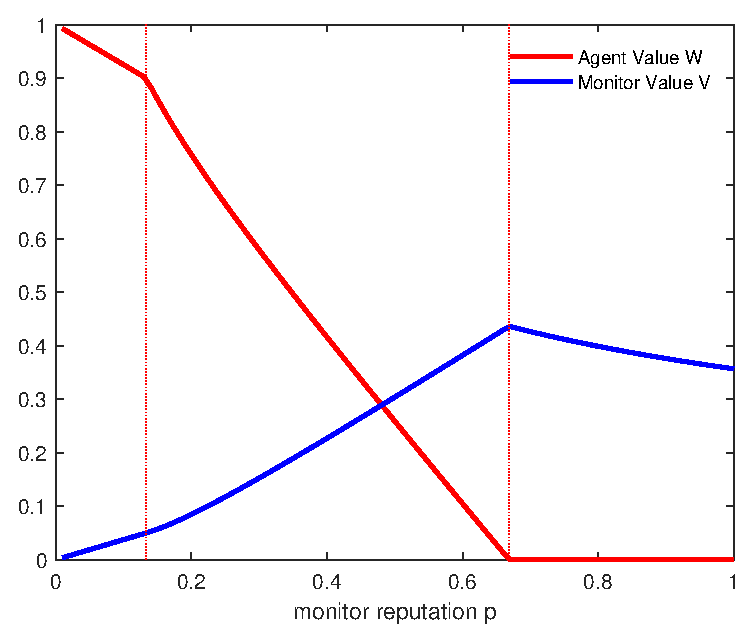
\includegraphics[scale=.6]{../code/fig-eq-presentation.eps}
\end{figure}
\hfill \hyperlink{frame:Prop1}{\beamerbutton{Back}}
\end{frame}


\begin{frame}{Non-Monotone Equilibria}\label{frame:OtherEq}
\begin{center}
        \begin{tikzpicture}[scale=\textwidth/12cm] 
        % draw horizontal line  
        \draw[->] (0,0) -- (11,0);  
        % draw vertical lines  
        \foreach \x in {0,3,10}  
        \draw (\x cm,3pt) -- (\x cm,-3pt); 
        % draw nodes  
        \draw (0,0) node[below=3pt,text width=1.5cm,align=center] {$0$}; 
        \draw (3,0) node[below=3pt,text width=1.5cm,align=center] {$p_l$}; 
        \draw (10,0) node[below=3pt,text width=1.5cm,align=center] {$1$}; 
        \draw (11,0) node[below=3pt,text width=1.5cm,align=center] {$p$};
        \draw[thick,red] (0,0)--(4.5,0);
        \draw[thick,red] (5.5,0)--(6.2,0);
        \draw[thick,red] (6.7,0)--(7.7,0);
        \end{tikzpicture}       
\end{center}

Monotonicity assumption rules those out\\
\bigskip
\hfill \hyperlink{frame:Prop1}{\beamerbutton{Back}}
\end{frame}

\begin{frame}{Small $R$: Monitor Never Exerts Effort}\label{frame:Small-R}
\begin{center}
        
        \begin{tikzpicture}[line cap=round,line join=round,>=triangle 45,x=1.0cm,y=1.0cm, domain=-1:10, range=-6:8] 
        
        \begin{axis}[
        axis x line=center, 
        axis y  line=center, 
        xmin = -1, xmax = 11, xtick = \empty, xlabel = $p$,
        ymin = -4, ymax = 8, ytick = \empty, ylabel = $ $,
        xlabel style = {at={(ticklabel cs:1)}},
        ylabel style = {at={(ticklabel cs:0.9)},anchor=near ticklabel},
        extra x ticks={4,6.25,7.5,10},
        extra x tick labels={,,,},
        extra y ticks={5},
        extra y tick labels={,},
        width=0.7\textwidth, 
        height=0.7\textwidth,
        legend style={nodes=right}, 
        legend pos= north east]
        
        \draw<1->[red,thick] (axis cs: 0,5) -- (axis cs: 6.25,0);
        \draw<1-2>[red,thick] (axis cs: 6.25,0) -- (axis cs: 10,-3);
        \draw<3->[red,thick] (axis cs: 6.25,-1) -- (axis cs: 10,-4);
        
%       \draw<1->[red,thick] (axis cs: 0,5) -- (axis cs: 4,1.8);
%       \draw<2->[red,thick] (axis cs: 4,2.2) to [out=-20,in=140] (axis cs: 5.5,1.5);
%       \draw<2->[red,thick] (axis cs: 5.5,1.5) to [out=-40,in=120] (axis cs: 7,0);
%       %       \draw<5->[red,thick] (axis cs:7,0) to [out=-70,in=160] (axis cs: 10,-2);
%       \draw<5->[red,thick] (axis cs:7,-1.5) to (axis cs: 10,-3.5);
        \addlegendimage{color=red};
        \addlegendentry{$\omega(p)$};
%       \node<4->[anchor=north] at (axis cs: 7,0) {$\bar{p}_h$};
        
        \draw<1>[blue,thick] (axis cs: 0,-2) -- (axis cs: 10,3);
        \draw<2>[blue,thick,dashed] (axis cs: 0,-2) -- (axis cs: 10,3);
        \draw<2>[blue,thick] (axis cs: 0,-3) -- (axis cs: 10,1);
        \draw<3->[blue,thick] (axis cs: 0,-3) -- (axis cs: 6.25,-0.5);
        \draw<3->[blue,thick] (axis cs: 6.25,-1.5) to [out=-50,in=170] (axis cs: 10,-3);
%       \draw<1->[blue,thick] (axis cs: 0,-2) -- (axis cs: 4,0);
%       \draw<3->[blue,thick] (axis cs: 4,0) to [out=50,in=220] (axis cs: 5.5,1.2);
%       \draw<3->[blue,thick] (axis cs: 5.5,1.2) to [out=30,in=190] (axis cs: 7,2);

        \addlegendimage{color=blue};
        \addlegendentry{$\gamma p V'(p)-c$};
        
        \node<1>[anchor=north] at (axis cs: 4,0) {$p_l$};
        
        \node<2>[anchor=north] at (axis cs: 7.5,0) {$p_l$};
        
        \node<3>[anchor=north] at (axis cs: 6.25,0) {$p_{nm}$};
        
        \node[anchor=north west] at (axis cs: 0,0) {$0$};
        \node[anchor=north] at (axis cs: 10,0) {$1$};
        
        
        \end{axis}      
        \end{tikzpicture} 
\end{center}
\only<1>{\centering{Construct equilibrium thresholds $p_l,p_h$}}
\only<2>{\centering{Not optimal to manipulate on $[0,p_l)$}}
\only<3>{\centering{No-monitoring equilibrium} \\}
\only<3>{\hfill \hyperlink{frame:End-Eq-Constr}{\beamerbutton{Back}}}
\end{frame}

\end{document}



